\chapter{پردازش‌های پایه جهت تشخیص اخبار جعلی برروی داده‌های فارسی}
\section{پیش‌پردازش داده‌های خبری}
یکی از مهم‌ترین بخش‌های تشخیص اخبار جعلی پیش‌پردازش داده‌های خبری است. پیش‌پردازش داده‌ها به معنی یک‌دست‌سازی واژه‌ها برای استفاده در الگوریتم‌های پردازش متن است که در ادامه مراحل آن را مرور می‌کنیم.
 

\subsection[هنجارسازی واژه‌ها]{هنجارسازی\LTRfootnote{Text normalization} واژه‌ها}
قبل از این که بتوان از این که مجموعه‌ای از متن‌ها به‌عنوان داده ورودی مورد استفاده الگوریتم‌های یادگیری قرار گیرد،  ابتدا باید پیش‌پردازش‌هایی روی آنها انجام گیرد تا صورت‌های غیرمعیار به شکل معیار تبدیل گردد. اگر حروف، نشانه‌های نگارشی و واژه‌های فارسی به شکل یکسانی نوشته نشود، مجموعه داده استفاده‌شده قابل تحلیل توسط سامانه‌های رایانه‌ای نخواهند بود. طی فرایند هنجارسازی، علایم نگارشی، حروف، فاصله‌های بین واژه‌ها و اختصارات  بدون ایجاد تغییرات معنایی در متن، به شکل استاندارد تبدیل می‌گردد. برای عنوان مثال، برخی از حروف در زبان فارسی به کدهای مختلف به چند شکل متفاوت نوشته می‌شود که باید به یک صورت یکسان تبدیل گردد، مانند انواع حروف «ک» در زبان فارسی و عربی و یا شکل‌های متفاوت نوشتاری حرف «ی» در فارسی، عربی و پشتو. همچنین در این مرحله تمامی اعراب‌ها مانند فتحه، کسره، ضمه  و تشدید از واژه‌ها حذف و یا به صورت استانداردی تبدیل می‌شود. ممکن است  علامت تنوین  ~ً~ در واژه‌ای مانند «حتماً» یا همزه آخر بعضی از واژه‌ها مانند «انشاء» حذف  شده باشد که برای کاهش تنوع نگارشی واژه‌ها و کوچک‌‌سازی واژگان هنجارسازی واژه‌ها انجام می‌پذیرد.


\subsection[واحدسازی واژه‌ها]{واحدسازی\LTRfootnote{Tokenization} واژه‌ها}
در زبان فارسی بعضی از حروف چهار شکل دارد که سه شکل آن به حرف مجاور چسبیده است و شکل دیگر منفصل است. مجموعه محدودی از حروف مانند «ا»، «د»، «ذ»، «ر»، «ز»، «ژ» و «و» فقط دارای دو شکل منفصل یا چسبیده به حرف قبلی را دارد. عدم چسبندگی این مجموعه محدود به حرف بعدی سبب می‌شود در هنگام نگارش  متن فاصله کامل به‌عنوان مرزنمای واژه وارد نشود و یک واحد به‌صورت یکپارچه نوشته شود، مانند ویابهتر است. اگرچه ممکن است زنجیره حروف در این مثال خوانش توسط انسان را دچار اختلال نکند، تمام زنجیره به‌عنوان یک واژه توسط رایانه تشخیص داده می‌شود.  نادیده‌گرفتن درج فاصله کامل در متن به‌خصوص متن‌های خبری که با سرعت تهیه و منتشر می‌شود اجتناب‌ناپذیر است.

هر خبر شامل مجموعه از جملات است که هر جمله نیز از مجموعه‌ای از واژه تشکیل شده‌ است. به‌منظور قابل‌فهم کردن اخبار برای الگوریتم‌های یادگیری ماشین و شبکه‌های عمیق باید هر جمله خبر به کوچک‌ترین جزء تشکیل‌دهنده که همان واژه‌ها است تجزیه شود. به این عمل قطعه‌بندی جملات می‌گویند. در زبان فارسی بسیاری از واژه‌های مرکب دارای نیم‌فاصله در درون واژه است که مانع چسبندگی حروف دردرون یک واژه می‌شود که به خوانش راحت‌تر آن توسط گویشور می‌انجامد، مانند فروشگاه‌ها. اما بسیاری از نوشته‌های کاربران و خبرگزاری‌ها از این قانون پیروی نمی‌کند. به‌عنوان مثال واژه‌هایی مانند «می نوشد»، «کتاب ها»، «بین الملل» که باید به ترتیب به‌صورت «می‌نوشد»، «کتاب‌ها» و «بین‌الملل» نوشته شود با فاصله کامل نوشته می‌شود. گاهی وجود فاصله کامل یا نیم‌فاصله به ابهام منجر می‌شود مانند «می نوشد» و «می‌نوشد» که رفع ابهام این موارد چندان ساده نیست. لازم به ذکر است ممکن است فاصله بین دو تکواژ حذف شود و صورت دیگری از نوشتار به‌دست آید، مانند علاقمند. بر اساس آنچه ذکر شد چنین می‌توان نتیجه گرفت که پیش از انجام هر عملیاتی برای تقطیع جملات به واژه‌ها، باید عملیات اصلاح این نگارش‌ها انجام شود.

\subsection[حذف ایست‌واژه‌ها و علائم نگارشی]{حذف ایست\LTRfootnote{Stop words} واژه‌ها و علائم نگارشی}
 ایست‌واژه‌ها مجموعه‌ای از واژه‌های پرکاربرد در یک حوزه است که معنای خاصی به جملات در آن حوزه اضافه نمی‌کند. به‌عنوان مثال تمامی حروف اضافه مانند «از»، «به» یا افعالی مانند «است» و «شد» جزو این مجموعه حساب می‌شود. علاوه بر این موارد، واژه‌هایی مانند «خبر»، و «خبرگزاری» در حوزه اخبار بسیار پرتکرار محسوب می‌شود و اطلاعات زیادی را شامل نمی‌شود. همچنین علائم نگارشی نیز باید در این مرحله از میان واژه‌ها حذف شود.
 
\subsection[ریشه‌یابی واژه‌ها]{ریشه‌یابی\LTRfootnote{Stemming} واژه‌ها}
هدف از ریشه‌یابی واژه‌ها حذف پیشوندها و پسوندها و رسیدن به ستاک\LTRfootnote{Stem} است که یافتن ستاک دو مقوله فعل و اسم از اهمیت زیادی برخوردار است؛ چراکه این دو مقوله درصد زیادی از واژگان زبان را شامل می‌شود. این مرحله به کاهش واژه‌ها مشابه کمک می‌کند؛ چراکه ممکن است صورت‌واژه‌های\LTRfootnote{Word form} متنوعی با کمک فرایندهای تصریف\LTRfootnote{Inflection} و اشتقاق\LTRfootnote{Derivation} از یک ستاک ساخته شود. به‌عنوان مثال «می‌خوانم» و «می‌خواند» صورت‌واژه‌های ستاک «خوان» است که باید به صورت یکسان فرض شود؛ بنابراین در این مرحله هر دو واژه به «خوان» تبدیل می‌شود. همچنین پسوندهای جمع مانند «ها» و «ان» نیز در این مرحله از واژه‌ها حذف می‌شود.

\section{استخراج ویژگی‌های موضوعی مستندات}
\label{section.cat}
علاوه بر استفاده از اطلاعات نحوی و معنایی واژگان می‌توان ویژگی‌های وابسته به موضوع مستندات را هم از متن اخبار استخراج کرد تا با کمک آن‌ها بتوان به دقت بالاتری در تشخیص اخبار جعلی رسید. یکی از ویژگی‌های مهم هر خبر، موضوع آن خبر است که کمک زیادی در تشخیص جعلی یا اصیل بودن آن‌ می‌کند. برای مثال، عمده اخبار جعلی در اخبار سیاسی است که با استفاده از ویژگی موضوع خبر می‌توانیم با دقت بیشتر جعلی‌بودن خبر را تشخیص دهیم. دو رویکرد برای بهره‌گیری از اطلاعات مربوط به موضوع اخبار فارسی در این پروژه مورد بررسی قرار گرفته است:
\begin{itemize}
	\item دسته‌بندی موضوعی با استفاده از روش‌های یادگیری با نظارت
	\item مدل‌سازی موضوعی با استفاده از روش‌های یادگیری بدون ‌نظارت
\end{itemize}

\subsection{دسته‌بندی بانظارت براساس 6 دسته مختلف}‌
موضوعات اخبار به دو صورت مشخص می‌شود. در یک حالت اخبار به صورت کلی به چند دسته اصلی تقسیم می‌شود و سپس در سطح دوم هر یک از این دسته‌ها به چند زیر دسته تقسیم می‌گردد. یکی از دسته‌بندی‌های استاندارد که در این زمینه وجود دارد، دسته‌بندی ارائه‌شده در پیکره همشهری است \citep{aleahmad2009hamshahri} که حاوی ۶ دسته کلی اخبار علمی و دانشگاهی، فرهنگی و هنری، سیاسی و اقتصادی، اجتماعی، بین‌المللی و ورزشی در این داده موجود است. برای دسته‌بندی اخبار بر اساس این ۶ دسته می‌توانیم از یک روش یادگیری بانظارت استفاده کنیم. همانند هر مسئله دسته‌بندی، مجموعه‌ای از اخبار شامل متن خبر و موضوع آن را به الگوریتم یادگیری می‌دهیم و پس از اتمام یادگیری، با استفاده از این مدل می‌توانیم موضوع اخبار جدید را تشخیص دهیم و از آن به‌عنوان ویژگی‌ای اضافه‌شده به بردار تعبیه متن خبر، استفاده کنیم. برای این منظور، در این پژوهش از دسته‌بندی با نظارت با استفاده از مدل ‌زبانی برت و برای آموزش مدل دسته‌بند از مجموعه اخبار همشهری که آمار آن در \tablename~\ref{table.hamshahri} آمده، ‌استفاده کرده‌ایم.
پس‌ از آموزش دسته‌بند، عملیات دسته‌بندی می‌تواند بر روی هر خبری انجام شود و حاصل این دسته‌بندی به‌صورت یک بردار تک‌روشنِ شش‌بُعدی نمایش داده شود تا از آن به‌عنوان ویژگی در آموزش مدل‌های تشخیص اخبار جعلی بهره برده شود.

\begin{table} [h!]
	\caption{آمار و اطلاعات مربوط به دادگان همشهری}
	\label{table.hamshahri}
	\begin{center}
		\begin{tabular}{|M{6cm}|M{4cm}|}
			\hline
				ویژگی & مقدار \\
			\hline
			\hline
			حجم دادگان & 564 مگابایت \\ \hline
			نوع اسناد & متن \\ \hline
			تعداد اسناد & $166,774$ \\ \hline
			تعداد واژه‌های یکتا & $417,339$ \\ \hline
			میانگین طول سند & 380 واژه \\ \hline
			تعداد دسته‌ها & 82 \\ \hline
			تعداد موضوعات & 65 \\ \hline
		\end{tabular}
	\end{center}
\end{table}

\subsection{دسته‌بندی بدون‌ نظارت براساس روش تخصیص نهان دیریکله}
\label{section.lda_classification}
روش تخصیص نهان دیریکله\LTRfootnote{Latent Dirichlet allocation (LDA)} \citep{blei2003latent} یک روش بدون‌ نظارت بر مبنای مدل‌های احتمالاتی است که در آن با دریافت  پیکره  اخبار، دسته‌های موضوعات مستندات را انتخاب می‌کند. هر دسته باتوجه ‌به هم‌نشینی واژه‌ها در پیکره متن مشخص می‌شود. بنابراین نماینده هر موضوع مجموعه‌ای از واژه‌ها خواهد بود که باید برچسب آن‌ها مشخص گردد. این روش  ۲ ماتریس خروجی تولید می‌کند:
\begin{itemize}
	\item
ماتریس واژه-موضوع، که نشان می‌دهد در هر موضوع استنتاج‌شده چه واژه‌هایی قرار دارد.
	\item
ماتریس سند-موضوع، که نشان‌دهنده آن است که هر سند چه سهمی از موضوعات مختلف را دارد. بیشترین سهم نشان‌دهنده موضوع اصلی آن سند خواهد بود.
\end{itemize}
یکی از چالش‌های اصلی این روش پیداکردن مقدار بهینه برای تعداد موضوعات است؛ چراکه اگر این مقدار خیلی زیاد شود، موضوعات نسبتاً مرتبط از یکدیگر جدا خواهند شد و خطای احتمالی برای پیش‌بینی یک خبر جدید بیشتر می‌شود. از طرف دیگر، اگر تعداد موضوعات خیلی کم انتخاب شود، موضوعات نامرتبط دارای یک برچسب موضوعی یکسان خواهد شد. یکی از راه‌های پیداکردن مقدار بهینه برای موضوعات اخبار درکنارِ داشتنِ آگاهی از مقدار حدودی تعداد موضوعات معمول در خبرگزاری‌ها، استفاده از تعدادی است که خطای کلی مدل به کمترین مقدار برسد. برای این منظور، چند عدد متفاوت برای مدل‌سازی موضوعی انتخاب خواهد شد و با بررسی خروجی مدل و ارزیابی کیفی، به‌صورت تجربی تعداد بهینه موضوعات مشخص می‌گردد.

\section{بازنمایی برداری اخبار با رویکردهای مختلف}
یکی از چالش‌های پردازش زبان طبیعی یافتن یک بازنمایی مناسب برای جملات و یا اجزای کوچکتر آن مانند واژه‌ها است. واژه علاوه بر صورت‌واژه که ازطریق خط تجلی عینی پیدا می‌کند، دارای معنا است که معنای واژه با توجه به بافتی که در آن ظاهر می‌شود تعیین می‌شود. مهم‌ترین عامل تأثیرگذار بر کیفیت یک بازنمایی، شیوه مدل‌سازی معنایی واژه‌ها و یا جملات است. هرچقدر حجم اطلاعات در این بازنمایی بیشتر باشد، بازنمایی دقیق‌تری از واژه یا جمله به‌دست می‌آید. در سال‌های اخیر بازنمایی‌های متفاوتی در حوزه پردازش زبان طبیعی معرفی شده ‌است. در ادامه به توضیح چهار نوع بازنمایی مختلف که به چهار حیطه مختلف اشاره دارد می‌پردازیم. این بازنمایی‌ها عبارت است از بازنمایی بسامد واژه-معکوس بسامد سند که نوعی بازنمایی پایه مبتنی‌بر واژه است، بازنمایی تعبیه ایستا ورد2وک که نوعی بازنمایی مبتنی‌بر معنا براساس بافت است، بازنمایی برت که نوعی بازنمایی مبتنی‌بر معنای بافت‌محور است و بازنمایی تخصیص نهان دیریکله که نوعی بازنمایی مبتنی‌بر موضوع است.

\subsection{بازنمایی مبتنی ‌بر واژه}
یکی از ساده‌ترین روش‌ها برای بازنمایی اخبار روش مبتنی‌بر واژه است. در این روش با استفاده از شمارش واژه‌های پراهمیت در یک پیکره متنی، یک بازنمایی از آن‌ پیکره ساخته می‌شود. این روش از دو بخش بسامد واژه و معکوس بسامد سند تشکیل شده‌است. بسامد واژه برابر است با تعداد دفعاتی که یک واژه در یک متن تکرار شده‌است. البته برای محاسبه این بسامد، فرمول‌های متنوعی وجود دارد. همچنین معکوس بسامد سند به معنای تعداد دفعاتی است که یک اصطلاح در اسناد دیگر به‌کار رفته‌است که همانند بسامد واژه، روش‌های متنوعی برای محاسبه این معیار وجود دارد که در \tablename~\ref{table.tf} و \ref{table.idf} آورده شده‌است. $N$ تعداد تمام اسناد، $n_t$ تعداد اسنادی که واژه $t$ در آنها وجود دارد.

\begin{table}[h!]
	\caption{روابط قابل استفاده برای محاسبه بسامد واژه در یک سند}
	\label{table.tf}
	\begin{center}
		\begin{tabular}{|M{5cm}|M{5cm}|}
			\hline
			رویه وزن‌دهی\footnotemark & وزن بسامد واژه \\
			\hline
			\hline
						دودویی\footnotemark & 
			$0, 1$ \\ \hline
						تعداد & 
			$f_{t, d}$ \\ \hline
						بسامد واژه & 
			$ \frac{f_{t,d}}{\sum_{t^{'} \in d} f_{t^{'}, d}}$ \\ \hline
						هنجارسازی لگاریتمی\footnotemark & 
			$\log(1 + f_{t, d})$ \\ \hline
						هنجارسازی دو نیم\footnotemark & 
			$0.5 + ‌0.5\cdot \frac{f_{t, d}}{\max_{t^{'} \in d}{f_{t^{'}, d}}} $ \\ \hline
						هنجارسازی دو کا\footnotemark & 
			$K + (1 - K) \cdot \frac{f_{t, d}}{\max_{t^{'} \in d}{f_{t^{'}, d}}} $ \\ \hline
		\end{tabular}
	\end{center}
\end{table}
\LTRfootnotetext[7]{Weighting scheme}
\LTRfootnotetext[8]{Binary}
\LTRfootnotetext[9]{Log normalization}
\LTRfootnotetext[10]{Double normalization 0.5}
\LTRfootnotetext[11]{Double normalization k}
\begin{table}[h!]
	\caption{روابط قابل استفاده جهت محاسبه معکوس بسامد سند}
	\label{table.idf}
	\begin{center}
		\begin{tabular}{|c|c|}
			\hline
			رویه وزن‌دهی & وزن معکوس بسامد سند \\
			\hline
			\hline
			یگانه & 
			$1$ \\ \hline
			معکوس بسامد سند & 
			$-\log \frac{n_t}{N}$ \\ \hline
			معکوس بسامد سند هموار & 
			$\log(\frac{N}{1 +‌n_t}) + 1$ \\ \hline
			معکوس بسامد سند بیش‌ترین & 
			$\log(\frac{\max_{t^{'} \in d} n_{t^{'}}}{1 +‌n_t})$ \\ \hline
			معکوس بسامد سند احتمالاتی & 
			$\frac{N - n_t}{n_t}$ \\ \hline
		\end{tabular}
	\end{center}
\end{table}

\subsection{بازنمایی مبتنی ‌بر تعبیه ایستا (ورد2وک)}
در روش مبتنی‌بر واژه،  بر اساس فراوانی و توالی واژه‌های استفاده‌شده در یک پیکره سعی می‌کنیم تا یک بازنمایی مناسب ایجاد کنیم. اما این بازنمایی ارتباط میان اجزای جمله را به‌صورت محدود مدل‌سازی می‌کند. در روش مبتنی‌بر تعبیه ایستا، با استفاده از یک پیکره بزرگ متنی، برای هر واژه یک بازنمایی در اندازه پنجره مشخص ساخته می‌شود. این بازنمایی تا حد قابل قبولی مفاهیم هر واژه را در ساخت بردار در نظر می‌گیرد. خروجی این شیوه بردارسازی به این صورت است که اگر با استفاده از ابزار مصورسازی و کاهش بُعد، یک تصویر از مجموعه واژه‌های یک پیکره را داشته باشیم، اسامی شهر و یا نام ورزش‌های مختلف در نزدیکی هم دیده خواهد شد. علاوه بر این، روابط منطقی نیز میان بردارهای واژه‌ها برقرار است، به‌عنوان مثال، تفاضل بردار واژه‌های «مرد» و «زن» با تفاضل بردار واژه‌های «پادشاه» و «ملکه» برابر است. در بازنمایی ورد2وک، واژه‌ها به فضای برداری نگاشت می‌شود. اگر نیاز به نگاشت اسناد باشد روش داک2وک\LTRfootnote{Doc2vec} و یا میانگین برداری ورد2وک مورد استفاده قرار می‌گیرد. الگوریتم مبتنی‌بر تعبیه ایستا از دو مدل کیسه‌واژه پیوسته\LTRfootnote{Continuous Bag of words} و پرش‌نگاشت\LTRfootnote{Skip-gram}\citep{mikolov2013distributed} استفاده می‌گردد که در ادامه به‌صورت خلاصه آنها را مرور می‌کنیم.

\subsubsection{مدل کیسه‌واژه پیوسته}
برای یادگیری بردار واژه‌ها از همنشینی واژگان در یک پنجره لغزان استفاده می‌شود. در مدل کیسه‌واژه پیوسته، یک واژه به‌عنوان واژه هدف انتخاب شده و به اندازه پنجره لغزان واژه‌های قبل و بعد آن در فرایند یادگیری بردار واژه هدف شرکت می‌کنند. در این مدل هر واژه با استفاده از بازنمایی تک‌روشن به یک شبکه عصبی با یک لایه میانی داده می‌شود و در خروجی انتظار داریم تا احتمال واژه هدف بیشتر از بقیه واژه‌ها باشد. به این صورت مدل  تلاش می‌کند تا واژه هدف را با استفاده از واژه‌های دیگر حدس بزند.

\subsubsection{مدل پرش‌نگاشت}
در مدل کیسه‌واژه پیوسته معنای برخی از واژه‌ها به درستی یادگرفته نمی‌شود؛ چراکه در این میان، تعداد بسیار زیادی از واژه‌های هم‌معنا محو خواهند شد. به همین دلیل، این مدل دقیقا برعکس مدل کیسه‌واژه پیوسته عمل می‌کند تا مشکل معنایی واژه‌های کم تکرار حل شود؛ به این شکل که مدل شبکه عصبی با یک لایه میانی، بردار واژه میانی را دریافت می‌کند و در خروجی، انتظار داریم تا واژه‌هایی که در بافت جایگاهی\LTRfootnote{Local context} اطراف واژه هدف در پنجره لغزان وجود دارد، پیش‌بینی گردد. بنابراین با کاهش هزینه در هر مرحله، مدل تلاش می‌کند تا باتوجه‌به روابط میان واژه‌ها، برداری را برای بازنمایی آنها در لایه میانی یاد بگیرد. ساختار این مدل در \figurename~\ref{fig.skipgram} آورده شده ‌است.

\begin{figure}[h!]
	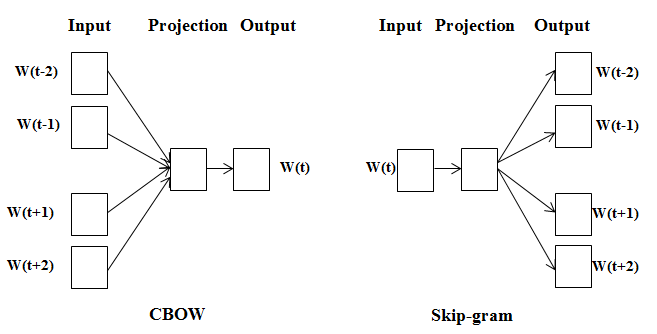
\includegraphics[width=1 \textwidth]{skipgram}
	\centering
	\caption{نمای کلی دو مدل پرش‌نگاشت و کیسه‌واژه پیوسته \citep{suleiman2017deep}}
	\label{fig.skipgram}
\end{figure}

\subsection{مبتنی ‌بر تعبیه بافت‌محور (برت)}
در بخش \ref{section.bert} با ساختار و روش آموزش مدل برت آشنا شدیم. شکل  \figurename \ref{fig.bert_embedding} 
ساختار این روش را نمایش می‌دهد.



\begin{figure}[!h]
	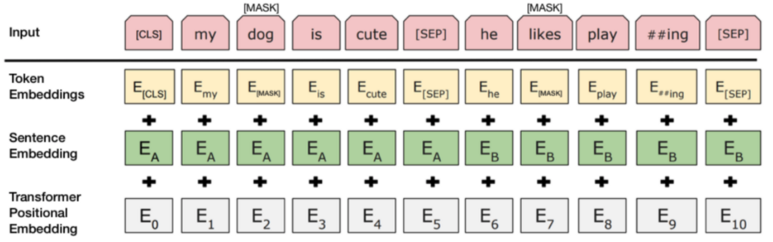
\includegraphics[width=1 \textwidth]{bert_embedding}
	\centering
	\caption{نحوه ترکیب تعبیه‌های سه‌گانه در مدل زبانی برت \citep{devlin2018bert}}
	\label{fig.bert_embedding}
\end{figure}



این مدل برای ایجاد یک بازنمایی مناسب از جملات از ترکیب سه تعبیه استفاده می‌کند که در ادامه توضیحات آنها ارائه می‌شود:
\begin{itemize}
	\item{تعبیه واژه \LTRfootnote{Token Embedding}}: منظور از تعبیه واژه تبدیل هر واژه به فضای برداری یکتا است.
	
	\item{تعبیه جمله \LTRfootnote{Sequence Embedding}}: هر داده ورودی مدل برت از دو جمله «آ» و «ب» تشکیل شده‌است که در یکی از مراحل یادگیری، این مدل برای پیش‌بینی جمله بعدی کاربرد دارد. به همین منظور، این مدل یک تعبیه برای مشخص‌کردن جمله‌ای که واژه مورد نظر در آن قرار دارد، ایجاد می‌کند.
	\item{تعبیه موقعیت انتقال‌دهنده‌ها \LTRfootnote{Transformer Positional Embedding}}: تعبیه موقعیت انتقال‌دهنده‌ها یک تعبیه از موقعیت هر واژه در جمله است که باعث می‌شود بردار حضور هر واژه در جایگاه‌های مختلف در یک جمله متفاوت باشد.
\end{itemize}

درنهایت با ترکیب این سه بخش، یک بردار ورودی برای مدل برت ساخته می‌شود که پس از مراحل یادگیری گفته‌شده در بخش قبل، برای هر جمله یک بازنمایی مناسب ارائه می‌یابد.


\subsection{بازنمایی مبتنی ‌بر موضوع (تخصیص نهان دیریکله)}
همان‌طور که در بخش \ref{section.lda_classification} بیان شد، الگوریتم تخصیص نهان دیریکله یک روش مدل‌سازی بدون‌نظارت برای تعیین موضوعات پیکره متنی است. روش عملکرد مدل‌سازی موضوع به این صورت است که پس از ورود پیکره به این الگوریتم، در نهایت ماتریس سند-موضوع و ماتریس واژه-موضوع ساخته می‌شود. به‌منظور استفاده از این روش برای یافتن یک بازنمایی مناسب برای هر سند می‌توانیم از ماتریس اول استفاده کنیم. هر سطر ماتریس سند-موضوع مرتبط با یک سند است و ستون آن احتمال هر موضوع را نشان می‌دهد. همچنین در ماتریس واژه-موضوع هر ستون یک موضوع است و هر سطر آن نیز امتیاز واژه در آن موضوع است.
